\documentclass{beamer}

\usepackage[english]{babel}
\usepackage[utf8]{inputenc}
\usepackage{listings}
%\usepackage{datetime}
\usepackage{graphics}
\usepackage{fancybox}
\usepackage{color}
\usepackage[normalem]{ulem}
\usepackage{hyperref}

\usepackage{tikz}
\usetikzlibrary{positioning}
\usepackage{hyperref}
\usetikzlibrary{shapes,arrows}

\usetheme{CambridgeUS}
%\usecolortheme{seagull}


\title{Osnove korištenja terminala}
\date{}
\author[Leonard Volarić Horvat]{Leonard Volarić Horvat \\ Antun Aleksa \\ Josip Žuljević}
\institute[ICM]{Istraživački centar mladih \\
				Fakultet elektrotehnike i računarstva}
				
\begin{document}
    %\beamerdefaultoverlayspecification{<+->}
{
\setbeamertemplate{headline}[] % still there but empty
\setbeamertemplate{footline}{}

\begin{frame}
\maketitle
\end{frame}
}

\begin{frame}
\frametitle{Sadržaj}
\tableofcontents
\end{frame}

\section{Operacijski sustav}
\begin{frame}[t]
\frametitle{Operacijski sustav}
  \begin{itemize}
    \setlength\itemsep{1em}
    \item Sučelje između hardvera i softvera
    \item Odvajanje detalja izvedbe hardvera od softvera
    \begin{footnotesize}
      \begin{itemize}
        \item Windows sustav se koristi na isti način neovisno o fizičkom računalu
      \end{itemize}
    \end{footnotesize}
    \item korisnik $\rightarrow$ aplikacija $\rightarrow$ OS $\rightarrow$ uređaj
  \end{itemize}
\end{frame}

\begin{frame}{Operacijski sustav}
Ilustracija: OS je sjeme
\begin{columns}[T]
    \begin{column}{.5\textwidth}
      \begin{figure}[h]
        \begin{minipage}{\textwidth}
          \centering
          \includegraphics[width=\linewidth]{peanut.jpg}
        \end{minipage}
      \end{figure}
    \end{column}

    \begin{column}{.5\textwidth}
      \begin{itemize}
        \item jezgra (\textit{kernel}) - pristup resursima
          \begin{footnotesize}
            \begin{itemize}
              \item upravljanje memorijom
              \item sinkronizacija procesa
              \item upravljanje vanjskim jedinicama - tipkovnica, miš, zvučnici...
              \item \dots
            \end{itemize}
          \end{footnotesize}
      
        \item ljuska (\textit{shell}) - "ono što korisnik vidi"
          \begin{footnotesize}
            \begin{itemize}
              \item \textbf{terminal}
              \item \textit{desktop environment}
              \item aplikacije - uređivači teksta, web preglednici
              \item \dots
            \end{itemize}
          \end{footnotesize}
      \end{itemize}
    \end{column}
  \end{columns}
\end{frame}


\section{Terminal}
\begin{frame}[c]
  \begin{center}
    \begin{Huge}
      Terminal
    \end{Huge}
  \end{center}
\end{frame}

\subsection{Vrste sučelja}

\begin{frame}[t]
\frametitle{Vrste sučelja}
  \begin{columns}
    \begin{column}{.7\textwidth}
      
    \textbf{CLI}
    \begin{itemize}
      %\setlength\itemsep{1em}
      \item Tekstualno naredbeno sučelje (\textit{Command Line Interface})
      \item Upis i ispis znakova koje ljuska interpretira kao naredbe
      \item Isključivo tekstualni ulaz/izlaz, liniju po liniju
      \begin{footnotesize}
        \begin{itemize}
          \item $\rightarrow$ \textbf{samo tipkovnica!}
        \end{itemize}
      \end{footnotesize}  
    \end{itemize}
    \vfill
    \textbf{GUI}
    \begin{itemize}
      %\setlength\itemsep{1em}
      \item Grafičko korisničko sučelje (\textit{Graphical User Interface})
      \item \textbf{Uvodi se koncept miša!}
      \item Bogatije, ali i kompleksnije rješenje
    \end{itemize}
    \end{column}
    \begin{column}{.3\textwidth}
      \begin{figure}[t]
        \begin{minipage}{\textwidth}
          \centering
          \includegraphics[width=\linewidth]{cli.png}
        \end{minipage}
      \end{figure}
      \begin{figure}[t]
        \begin{minipage}{\textwidth}
          \centering
          \includegraphics[width=\linewidth]{gui.png}
        \end{minipage}
      \end{figure}
    \end{column}
  \end{columns}
\end{frame}

\subsection{Terminal}
\begin{frame}[t]
\frametitle{Terminal}
  \begin{itemize}
    \setlength\itemsep{1em}
    \item Osnovni CLI ulazno-izlazni program
    \item Upis i ispis znakova koje ljuska interpretira kao naredbe
    \item Osnovna sintaksa: $<$ime\_naredbe$>$ [$<$zastavice$>$] [$<$argumenti$>$]
  \end{itemize}
  
  \vfill
  \begin{footnotesize}
    \begin{itemize}
      \item Nekad fizički uređaj za pristup ljusci
      \item Danas program koji simulira fizički uređaj
    \end{itemize}
  \end{footnotesize}  
\end{frame}

\begin{frame}[c]
  \begin{center}
    \begin{Huge}
      Datoteke i direktoriji
    \end{Huge}
  \end{center}
\end{frame}

\section{Direktoriji}
\subsection{Direktoriji}
\begin{frame}[t]
\frametitle{Direktoriji}
  \begin{itemize}
    \item Direktoriji su organizirani kao stablo (FHS - Filesystem Hierarchy Standard)
    \item U Unix operacijskom sustavu nema diskova
    \begin{itemize}
      \item Sve je \textbf{jedno} stablo direktorija s \textbf{jednim} 
            korijenom
    \end{itemize}
    \centering
    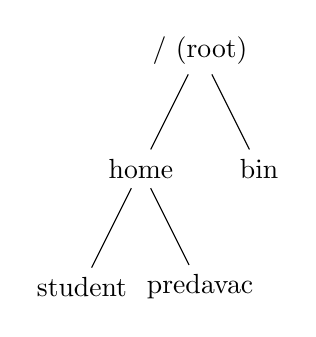
\begin{tikzpicture}
      \node {/ (root)}
          child { 
            node {home} 
            child {node {student} }
            child {node {predavac} }
          }
          child { node {bin} }
      ;
    \end{tikzpicture}
  \end{itemize}
\end{frame}

\begin{frame}[t]
\frametitle{Posebni direktoriji}
\begin{itemize}
  \item Svaki direktorij sadrži dva posebna direktorija
  \begin{itemize}
    \item \textit{..} roditeljski direktorij (engl. \textit{parent directory})
    \item \textit{.} trenutni direktorij (engl. \textit{current directory})
  \end{itemize}
  \item Primjeri
  \begin{itemize}
    \item \textit{ls . } 
    \begin{itemize}
      \item Ispisuje sadržaj trenutnog direktorija (uobičajeno \textit{ls} ponašanje)
    \end{itemize}
    \item \textit{ls .. }
    \begin{itemize}
      \item Ispisuje sadržaj direktorija koji je roditelj trenutnom
    \end{itemize}
  \end{itemize}
  \item Koriste se za \textbf{relativno} adresiranje direktorija
  \vfill
  \item Dva oblika staze (\textit{path}) do datoteke:
  \begin{itemize}
    \item \textbf{apsolutna} staza: cijeli put od roota do ciljane datoteke
    \item \textbf{relativna} staza: put od trenutnog direktorija do ciljane datoteke
  \end{itemize}
\end{itemize}
\end{frame}

\begin{frame}[t]
\frametitle{Pregled direktorija sustava}
  \begin{flushleft}
%  \includegraphics[scale=0.5]{filesystem}
  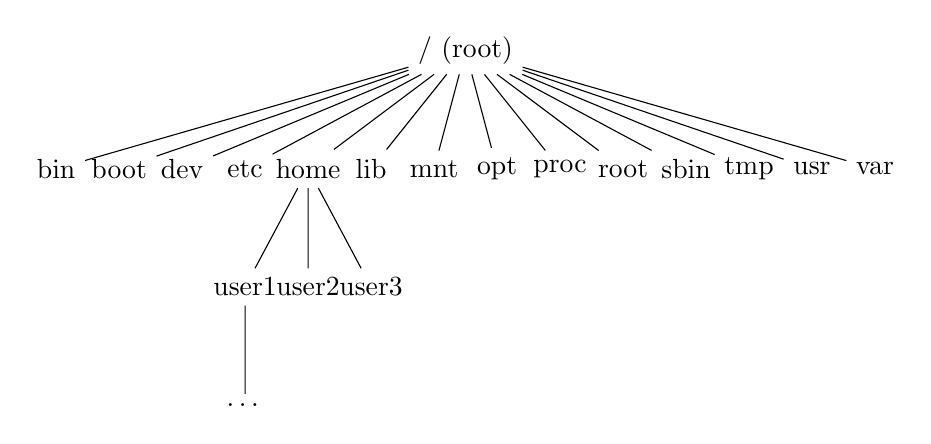
\begin{tikzpicture}[
      level 1/.style={sibling distance=8mm},
      level 2/.style={sibling distance=10mm}
      level 3/.style={sibling distance=12mm}
    ]
    \node {/ (root) }
        child {
          node {bin}
        }
        child {
          node {boot}
        }
        child {
          node {dev}
        }
        child {
          node {etc}
        }
        child {
          node {home}
          child {
            node {user1}
            child {
              node {\dots}
            }
          }
          child {
            node {user2}
          }
          child {
            node {user3}
          }
        }
        child {
          node {lib}
        }
        child {
          node {mnt}
        }
        child {
          node {opt}
        }
        child {
          node {proc}
        }
        child {
          node {root}
        }
        child {
          node {sbin}
        }
        child {
          node {tmp}
        }
        child {
          node {usr}
        }
        child {
          node {var}
        }
      ;
    \end{tikzpicture}
  \end{flushleft}
\end{frame}

\subsection{Datoteke}
\begin{frame}[t]
\frametitle{Datoteke}
  \begin{itemize}
    \item \textit{Everything is a file!}
    \item Na Unix sustavima je sve neka vrsta datoteke
      \begin{itemize}
        \item "obične" datoteke
        \item direktoriji
        \item blokovski uređaji - diskovi, USB stickovi
        \item znakovni uređaji - zvučne i grafičke kartice, tipkovnice
        \item mrežni socketi
        \item \dots
      \end{itemize}
    \vfill
    \item Imenovanje: 
    \begin{itemize}
      \item u imenu ne smije biti znak /
      \item datoteka se smatra skrivenom ako počinje točkom: .test
      \item ekstenzija (.txt, .sh, .py, .java...) je tek konvencija i nije nužna za funkcionalnost
    \end{itemize}
  \end{itemize}
\end{frame}



\begin{frame}[c]
  \begin{center}
    \begin{Huge}
      Osnovne naredbe
    \end{Huge}
  \end{center}
\end{frame}

\section{Osnovne naredbe}
\begin{frame}[t]
\frametitle{Osnovne naredbe za snalaženje po FHS}
  \begin{itemize}
    %\setlength\itemsep{1em}
    \item \textbf{ls} - ispis sadržaja direktorija
    \item \textbf{pwd} - ispis trenutnog direktorija
    \item \textbf{cd} - promjena direktorija
    \item \textbf{ls} - ispis sadržaja direktorija
    \item \textbf{cat} - ispis sadržaja datoteke
    \item \textbf{touch} - stvaranje prazne datoteke
    \item \textbf{mkdir} - stvaranje novog direktorija
    \item \textbf{rm(dir)} - brisanje datoteke (direktorija)
    \vfill
    \item \textbf{\underline{man}} - ispis detaljnih informacija o naredbi
  \end{itemize}
\end{frame}


\subsection{Primjeri i zadaci}

\begin{frame}[t]
\frametitle{Primjeri}
  \begin{enumerate}
    \item Pozicionirajte se u svoj direktorij Pictures
    \begin{itemize}
      \item apsolutno: \textit{cd /home/$<$username$>$/Pictures}
      \item ili, ako smo u matičnom direktoriju, relativno: \textit{cd Pictures}
    \end{itemize}
    \item Ispišite trenutni direktorij
    \item Stvorite direktorij "Black Mesa" (s razmakom u imenu!)
    \begin{itemize}
      \item \textit{mkdir Black Mesa}
    \end{itemize}
    \item Uđite u taj direktorij, uvjerite se da je prazan, pa se, koristeći relativnu stazu, pozicionirajte u svoj direktorij Music
  \end{enumerate}
\end{frame}


\begin{frame}[t]
\frametitle{Zadaci za vježbu}
  \begin{enumerate}
    \setlength\itemsep{1em}
    \item Pozicionirajte se u svoj direktorij Desktop
    \item Stvorite direktorij Hitchhiker
    \item U njemu stvorite datoteke Marvin, Hactar i .Magrathea (s točkom!)
    \item Ispišite \textbf{cijeli} sadržaj direktorija
    \item Koristeći relativnu stazu, pozicionirajte se u svoj direktorij Documents
    \item \textbf{Jednom naredbom} (hint: man mkdir) napravite direktorij Verse i u njemu direktorij Serenity
    \item Koristeći kratki izraz za matični direktorij (\textasciitilde), vratite se u njega i jednom naredbom obrišite direktorij Hitchhiker zajedno s njegovim sadržajem
  \end{enumerate}
\end{frame}

\section{Upravljanje datotekama}
\begin{frame}[c]
  \begin{center}
    \begin{Huge}
      Upravljanje datotekama
    \end{Huge}
  \end{center}
\end{frame}

\begin{frame}[t]
\frametitle{Upravljanje datotekama}
  Premještanje:
  \begin{itemize}
    \item \textbf{mv} - premještanje i preimenovanje datoteke
    \item \textbf{cp} - kopiranje datoteke
  \end{itemize}
  Podaci o datoteci:
  \begin{itemize}
    \item \textbf{file} - ispis tipa datoteke (po aplikaciji za pristup!)
    \item \textbf{ls -l $<$ime\_datoteke$>$} - detaljni podaci o datoteci
    \item \textbf{stat} - (drugi) detaljni podaci o datoteci
  \end{itemize}

  Ispis:
  \begin{itemize}
    \item \textbf{cat} - ispis cijele datoteke
    \item \textbf{less} - uredniji ispis cijele datoteke koji podržava listanje (\textit{scrolling})
    \item \textbf{head} - ispis prvih \textit{n} linija datoteke
    \item \textbf{tail} - ispis zadnjih \textit{n} linija datoteke
    \item \textbf{grep $<$riječ$>$ $<$datoteka$>$} - traženje pojavljivanja riječi u datoteci
  \end{itemize}
\end{frame}

\section{Filteri, tokovi i cjevovodi}
\begin{frame}[t]
\frametitle{Filteri, tokovi i cjevovodi}
\begin{itemize}
  \item Svaki program na Linuxu ima definirane sljedeće ulaze i izlaze:
  \begin{itemize}
    \item Standardni ulaz (stdin)
    \item Standardni izlaz (stdout)
    \item Standardni izlaz za greške (stderr)
  \end{itemize}
  \item Svi su ti ulazi i izlazi vezani na terminal
  \begin{itemize}
    \item Ako ih nismo preusmjerili uz pomoć specijalnih operatora
  \end{itemize}
\end{itemize}
\end{frame}


\begin{frame}[t]
\frametitle{Primjer naredbe \textit{cat}}
\begin{itemize}
  \item Grafička ilustracija izlaza i ulaza
  \vspace{1cm}
  \tikzstyle{plaintext}=[thick]
  \tikzstyle{block}=[rectangle,draw=black!50,fill=black!20,thick]
  \begin{tikzpicture}[auto, >=latex',node distance=4.5cm]
    \node[plaintext]  (a)               {tipkovnica};
    \node[block]      (b) [right of=a,inner sep=1cm,inner ysep=4mm]  {cat};
    \node[plaintext]  (c) [right of=b]  {zaslon};
    \draw[->] (a) edge node {stdin} (b);
    \draw[->] (b) edge node {stdout} (c);
  \end{tikzpicture}
  \vspace{1cm}
  \item Naredba \textit{cat} je filter!
  \begin{itemize}
    \item Preuzima nešto na ulazu
    \item Filtrira preuzete podatke
    \item Proslijeđuje rezultat na standardni izlaz
  \end{itemize}
\end{itemize}
\end{frame}

\subsection{Preusmjeravanje}
\begin{frame}[t]
\frametitle{Preusmjeravanje}
  Postoji nekoliko operatora za preusmjeravanje tokova:
  \begin{itemize}
    \item $<$ - preusmjeravanje sadržaja datoteke na \textit{input} naredbe
    \item $>$ - preusmjeravanje \textit{outputa} naredbe u datoteku
    \item $>>$ - preusmjeravanje \textit{outputa} naredbe na kraj datoteke
    \item $|$ (\textit{pipe}) - preusmjeravanje \textit{outputa} naredbe na \textit{input} iduće naredbe
  \end{itemize}
\end{frame}


\subsection{Primjeri i zadaci}
\begin{frame}[t]
\frametitle{Primjeri}
  \begin{itemize}
    \item Napravite prazne datoteke \textit{Wash} i \textit{Zoe}
    \item Koristeći naredbu \textit{echo}, upišite u datoteku Wash jednu liniju teksta
    \item Na isti način dodajte još jednu liniju, ali tako da očuvate i prethodni sadržaj
    \item Koristeći neki \textit{text editor}, upišite u datoteku \textit{Wash} 10 redova, a u \textit{Zoe} 5 redova teksta
    \item Obje datoteke premjestite u direktorij \textit{Verse/Serenity} iz prethodnog zadatka
    \item Ispišite prva 3 reda datoteke \textit{Zoe}
    \item Koristeći opciju za negativan broj redaka ispišite prvih 7 redova datoteke \textit{Wash}
    \item Ispišite druga 3 reda datoteke Wash
  \end{itemize}
\end{frame}




\begin{frame}[t]
\frametitle{Zadaci}
  \begin{itemize}
    \item Pozicionirajte se u direktorij \textit{/usr/share/dict}
    \item Provjerite postoji li u datoteci \textit{words} riječ "wiener" (hint: naredba grep!)
    \item Učinite isto za riječ "poslovanje"
    \item Provjerite koliko se puta u \textbf{drugih} 100 linija pojavljuje niz znakova "ga"
  \end{itemize}
\end{frame}


\section{Skripte}
\begin{frame}[c]
  \begin{center}
    \begin{Huge}
      Skripte
    \end{Huge}
  \end{center}
\end{frame}


\begin{frame}[t]
\frametitle{Skripte}
  \begin{itemize}
    \setlength\itemsep{1em}
    \item Niz naredbi zapisan u tekstualnu datoteku
    \item Zapisane se naredbe jednostavno slijedno izvode
    \item Ime skripte obično završava na .sh
    \vfill
    \item Za pokretanje potrebno imati \textbf{dozvolu za izvršavanje} -- \textit{chmod +x skripta.sh}
    \item Pokretanje skripte: ./skripta.sh
  \end{itemize}
\end{frame}


\subsection{Primjeri i zadaci}
\begin{frame}[t]
\frametitle{Primjer}
  \#!/bin/bash \\ mkdir alpha\_quadrant \\ cd alpha\_quadrant \\ touch \{betazed,earth,kronos,omicron\_theta,vulcan\} \\ echo "Before: " \\ ls -lh \\ echo "Live long and prosper" $>$ vulcan \\ echo "After: " \\ ls -lh \\ echo "So long and thanks for all the fish!"
\end{frame}



\begin{frame}[t]
\frametitle{Zadatak}
  Napisati skriptu koja:
  \begin{itemize}
    \item Stvara direktorij \textit{/tmp/my\_boot} i pozicionira se u nju
    \item Iz izlaza naredbe \textit{dmesg} uzima sve linije u kojima se pojavljuje riječ "boot" i sprema to u datoteku "original"
    \item Obrće poredak tih linija (koristeći prikladan oblik naredbe \textit{sort}) i rezultat te operacije sprema u "reverse"
    \item Miče prvu liniju iz datoteke "original" i sprema tu promjenu
    \item Ispisuje detalje o sadržaju direktorija
    \item Pozdravlja korisnika porukom "Bok!"
    \item Briše direktorij my\_boot i sav njegov sadržaj
  \end{itemize}
\end{frame}


\section{Package Manager}
\begin{frame}[t]
\frametitle{Upravljanje paketima}
\begin{itemize}
  \item paket je program
  \item \textit{yum, apt, pacman, zypper \ldots}
  \item Primjer naredbi za apt:
  \begin{itemize}
    \item  \textit{apt update}
  \item \textit{apt install sl}
  \end{itemize}
  \item Najčešće nužno koristiti administratorske ovlasti $\rightarrow$ \textbf{sudo}
  \item \textbf{sudo} - naredba koja privremeno daje administratorske ovlasti
\end{itemize}
\end{frame}

\begin{frame}[c]
\frametitle{Zadatak}
  \begin{center}
    \begin{huge}
    Instalirati git!
    \end{huge}
  \end{center}
\end{frame}

\begin{frame}[c]
  \begin{center}
    \begin{large}
    Hvala na pažnji!
    \end{large}
  \end{center}
\end{frame}


\end{document}
